\subsection{Теорема о полноте метода резолюций: из невыполнимой КНФ всегда можно вывести $\perp$.}

\textbf{Теорема.} Метод резолюций всегда заканчивает свою работу, причём для невыполнимых КНФ выводится $\perp$ (полнота), а для выполнимых не выводится (корректность).

\textbf{Доказательство.}

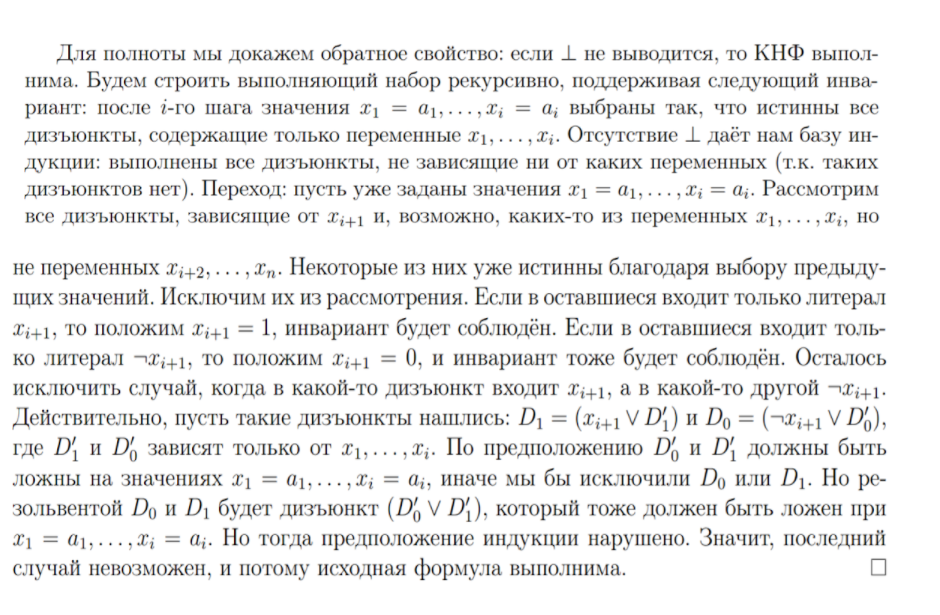
\includegraphics[width=0.9\textwidth]{images/1.4}